% Options for packages loaded elsewhere
\PassOptionsToPackage{unicode}{hyperref}
\PassOptionsToPackage{hyphens}{url}
%
\documentclass[
  a4paper,
]{article}
\usepackage{lmodern}
\usepackage{amssymb,amsmath}
\usepackage{ifxetex,ifluatex}
\ifnum 0\ifxetex 1\fi\ifluatex 1\fi=0 % if pdftex
  \usepackage[T1]{fontenc}
  \usepackage[utf8]{inputenc}
  \usepackage{textcomp} % provide euro and other symbols
\else % if luatex or xetex
  \usepackage{unicode-math}
  \defaultfontfeatures{Scale=MatchLowercase}
  \defaultfontfeatures[\rmfamily]{Ligatures=TeX,Scale=1}
\fi
% Use upquote if available, for straight quotes in verbatim environments
\IfFileExists{upquote.sty}{\usepackage{upquote}}{}
\IfFileExists{microtype.sty}{% use microtype if available
  \usepackage[]{microtype}
  \UseMicrotypeSet[protrusion]{basicmath} % disable protrusion for tt fonts
}{}
\makeatletter
\@ifundefined{KOMAClassName}{% if non-KOMA class
  \IfFileExists{parskip.sty}{%
    \usepackage{parskip}
  }{% else
    \setlength{\parindent}{0pt}
    \setlength{\parskip}{6pt plus 2pt minus 1pt}}
}{% if KOMA class
  \KOMAoptions{parskip=half}}
\makeatother
\usepackage{xcolor}
\IfFileExists{xurl.sty}{\usepackage{xurl}}{} % add URL line breaks if available
\IfFileExists{bookmark.sty}{\usepackage{bookmark}}{\usepackage{hyperref}}
\hypersetup{
  pdftitle={MATH2750 Introduction to Markov Processes},
  pdfauthor={Matthew Aldridge},
  hidelinks,
  pdfcreator={LaTeX via pandoc}}
\urlstyle{same} % disable monospaced font for URLs
\usepackage[margin=1in]{geometry}
\usepackage{longtable,booktabs}
% Correct order of tables after \paragraph or \subparagraph
\usepackage{etoolbox}
\makeatletter
\patchcmd\longtable{\par}{\if@noskipsec\mbox{}\fi\par}{}{}
\makeatother
% Allow footnotes in longtable head/foot
\IfFileExists{footnotehyper.sty}{\usepackage{footnotehyper}}{\usepackage{footnote}}
\makesavenoteenv{longtable}
\usepackage{graphicx,grffile}
\makeatletter
\def\maxwidth{\ifdim\Gin@nat@width>\linewidth\linewidth\else\Gin@nat@width\fi}
\def\maxheight{\ifdim\Gin@nat@height>\textheight\textheight\else\Gin@nat@height\fi}
\makeatother
% Scale images if necessary, so that they will not overflow the page
% margins by default, and it is still possible to overwrite the defaults
% using explicit options in \includegraphics[width, height, ...]{}
\setkeys{Gin}{width=\maxwidth,height=\maxheight,keepaspectratio}
% Set default figure placement to htbp
\makeatletter
\def\fps@figure{htbp}
\makeatother
\setlength{\emergencystretch}{3em} % prevent overfull lines
\providecommand{\tightlist}{%
  \setlength{\itemsep}{0pt}\setlength{\parskip}{0pt}}
\setcounter{secnumdepth}{5}
\usepackage{booktabs}

\usepackage{titlesec, environ}
\newif\ifcomm\commtrue
\NewEnviron{myanswers}{\ifcomm\BODY\fi}

\newcommand{\sectionbreak}{\clearpage}
\usepackage[]{natbib}
\bibliographystyle{plainnat}

\title{MATH2750 Introduction to Markov Processes}
\author{\href{mailto:m.aldridge@leeds.ac.uk}{Matthew Aldridge}}
\date{University of Leeds, 2020--2021}

\usepackage{amsthm}
\newtheorem{theorem}{Theorem}[section]
\newtheorem{lemma}{Lemma}[section]
\newtheorem{corollary}{Corollary}[section]
\newtheorem{proposition}{Proposition}[section]
\newtheorem{conjecture}{Conjecture}[section]
\theoremstyle{definition}
\newtheorem{definition}{Definition}[section]
\theoremstyle{definition}
\newtheorem{example}{Example}[section]
\theoremstyle{definition}
\newtheorem{exercise}{Exercise}[section]
\theoremstyle{remark}
\newtheorem*{remark}{Remark}
\newtheorem*{solution}{Solution}
\begin{document}
\maketitle

{
\setcounter{tocdepth}{2}
\tableofcontents
}
\hypertarget{home}{%
\section*{Schedule}\label{home}}
\addcontentsline{toc}{section}{Schedule}

\textbf{Week 1} (25--29 January)

\begin{itemize}
\tightlist
\item
  \protect\hyperlink{S00-about}{About the module}
\item
  \protect\hyperlink{S01-stochastic-processes}{\textbf{Section 1}: Stochastic processes and the Markov property}
\item
  \protect\hyperlink{S02-random-walk}{\textbf{Section 2}: Random walks}
\item
  \protect\hyperlink{P01}{\textbf{Problem Sheet 1}}
\item
  \textbf{Lecture}: Tuesday at 1400 (link in Minerva)
\item
  \textbf{Drop-in sessions}: Tuesday or Wednesday (Teams)
\end{itemize}

\hypertarget{S00-about}{%
\section*{About MATH2750}\label{S00-about}}
\addcontentsline{toc}{section}{About MATH2750}

This module is \textbf{MATH2750 Introduction to Markov Processes}. The module manager and lecturer is Dr Matthew Aldridge, and my email address is \href{mailto:m.aldridge@leeds.ac.uk}{\nolinkurl{m.aldridge@leeds.ac.uk}}.

\hypertarget{about-module}{%
\subsection*{Organisation of MATH2750}\label{about-module}}
\addcontentsline{toc}{subsection}{Organisation of MATH2750}

This module lasts for 11 weeks. The first nine weeks run from 25 January to 26 March, then we break for Easter, and then the final two weeks run from 26 April to 7 May.

\hypertarget{notes}{%
\subsubsection*{Notes and videos}\label{notes}}
\addcontentsline{toc}{subsubsection}{Notes and videos}

The main way I expect you to learn the material for this course is by reading these notes and by watching the accompanying videos. I will set two sections of notes each week, for a total of 22 sections.

Reading mathematics is a slow process. Each section roughly corresponds to one lecture last year, which would have been 50 minutes. If you find yourself regularly getting through sections in much less than an hour, you're probably not reading carefully enough through each sentence of explanation and each line of mathematics, including understanding the motivation as well as checking the accuracy.

It is possible (but not recommended) to learn the material by only reading the notes and not watching the videos. It is not possible to learn the material by only watching the videos and not reading the notes.

You are probably reading the web version of the notes. If you want a PDF copy (to read offline or to print out), then click the PDF button in the top ribbon of the page. (Warning: I have not made as much effort to make the PDF neat and tidy as I have the web version.)

Since we will all be relying heavily on these notes, I'm even more keen than usual to hear about errors mathematical, typographical or otherwise. Please, please \href{mailto:m.aldridge@leeds.ac.uk}{email me} if think you may have found any.

\hypertarget{problem-sheets}{%
\subsubsection*{Problem sheets}\label{problem-sheets}}
\addcontentsline{toc}{subsubsection}{Problem sheets}

There will be 10 problem sheets; Problem Sheet \(n\) covers the material from the two sections from week \(n\) (Sections \(2n -1\) and \(2n\)), and will be discussed in your workshop in week \(n+1\).

\hypertarget{lectures}{%
\subsubsection*{Lectures}\label{lectures}}
\addcontentsline{toc}{subsubsection}{Lectures}

There will be one online synchronous ``lecture'' session each week, on Tuesdays at 1400, with me, run through Zoom.

This will not be a ``lecture'' in the traditional sense of the term, but will be an opportunity to re-emphasise material you have already learned from notes and videos, to give extra examples, and to answer common student questions, with some degree of interactivity.

I will assume you have completed all the work for the previous week by the time of the lecture, but I will not assume you've started the work for that week itself.

I am very keen to hear about things you'd like to go through in the lectures; please \href{mailto:m.aldridge@leeds.ac.uk}{email me} with your suggestions.

\hypertarget{workshops}{%
\subsubsection*{Workshops}\label{workshops}}
\addcontentsline{toc}{subsubsection}{Workshops}

There will be 10 workshops, starting in the second week. The main goal of the workshops will be to go over your answers to the problems sheets in smaller classes. You will have been assigned to one of three workshop groups, meeting on Mondays or Tuesdays, led by \href{https://eps.leeds.ac.uk/maths/pgr/8790/jason-klebes}{Jason Klebes}, \href{http://www1.maths.leeds.ac.uk/~voss/}{Dr Jochen Voss}, or me. Your workshop will be run through Zoom or Microsoft Teams; your workshop leader will contact you before the end of this week with arrangements.

My recommended approach to problem sheets and workshops is the following:

\begin{itemize}
\tightlist
\item
  Work through the problem sheet before the workshop, spending plenty of time on it, and making multiple efforts at questions you get stuck on. I recommend spending \emph{at least three hours} on each problem sheet, in more than one block. Collaboration is encouraged when working through the problems, but I recommend writing up your work on your own.
\item
  Take advantage of the smaller group setting of the workshop to ask for help or clarification on questions you weren't able to complete.
\item
  After the workshop, attempt again the questions you were previously stuck on.
\item
  If you're still unable to complete a question after this second round of attempts, \emph{then} consult the solutions.
\end{itemize}

\hypertarget{assessments}{%
\subsubsection*{Assessments}\label{assessments}}
\addcontentsline{toc}{subsubsection}{Assessments}

There will be four pieces of assessed coursework, making up a total of 15\% of your mark for the module. Assessments 1, 2 and 4 will involve writing up answers to a few problems, in a similar style to the problem sheets, and are worth 4\% each. (In response to previous student feedback, there are fewer questions per assessment.) Assessment 3 will be a report on some computational work (\protect\hyperlink{about--computing}{see below}) and is worth 3\%.

While you may want to discuss an assessment with others in advance of completing it by yourself, copying is not allowed and will be dealt with in accordance with University rules.

The assessments deadlines are:

\begin{itemize}
\tightlist
\item
  Assessment 1: Thursday 11 February 1400 (week 3)
\item
  Assessment 2: Thursday 18 March 1400 (week 8)
\item
  Assessment 3 (Computing Worksheet 2): Thursday 25 March 1400 (week 9)
\item
  Assessment 4: Thursday 6 May 1400 (week 11)
\end{itemize}

Work will be submitted via Gradescope.

\hypertarget{about-computing}{%
\subsubsection*{Computing worksheets}\label{about-computing}}
\addcontentsline{toc}{subsubsection}{Computing worksheets}

There will be two computing worksheets, which will look at the material in the course through simulations in R. This material is examinable. You should be able to work through the worksheets in your own time, but if you need help, there will be optional online drop-in sessions in the weeks 4 and 7 with \href{https://eps.leeds.ac.uk/maths/pgr/6422/muyang-zhang}{Muyang Zhang} through Microsoft Teams. (Your computing drop-in session may be listed as ``Practical'' on your timetable.)

The first computing worksheet will be a practice run, while a report on the second computing worksheet will be the third assessed piece of work.

\hypertarget{dropin}{%
\subsubsection*{Drop-in sessions}\label{dropin}}
\addcontentsline{toc}{subsubsection}{Drop-in sessions}

If you there is something in the course you wish to discuss in detail, the place for the is the optional weekly drop-in session. You will have been assigned to one of three groups on Tuesdays or Wednesdays with \href{https://eps.leeds.ac.uk/maths/pgr/4992/nikita-merkulov}{Nikita Merkulov} or me. The drop-in sessions will be run the Microsoft Teams. Your drop-in session would be an excellent place to go if you are having trouble understanding something in the written notes, or if you're still truggling on a problem sheet question after your workshop.

\hypertarget{team}{%
\subsubsection*{Microsoft Team}\label{team}}
\addcontentsline{toc}{subsubsection}{Microsoft Team}

I have set up \href{https://teams.microsoft.com/l/channel/19\%3a8cb8008c95204bbeaefa8ee7d48c1a13\%40thread.tacv2/General?groupId=1c138eac-0c54-43b0-9d20-d4cf3d65c40a\&tenantId=bdeaeda8-c81d-45ce-863e-5232a535b7cb}{a Microsoft Team} for the course. I propose to use the ``Q and A'' channel there as a discussion board. This is a good place to post questions about material from the course, and -- even better! -- to help answer you colleagues' questions. The idea is that you all as a group should help each other out. I will visit a couple of times a week to clarify if everybody is stumped by a question, or if there is disagreement.

\hypertarget{time}{%
\subsubsection*{Time management}\label{time}}
\addcontentsline{toc}{subsubsection}{Time management}

It is, of course, up to you how you choose to spend your time on this module. But, if you're interested, my recommendations would be something like this:

\begin{itemize}
\tightlist
\item
  \textbf{Every week:} 7.5 hours per week

  \begin{itemize}
  \tightlist
  \item
    \textbf{Notes and videos:} 2 sections, 1 hour each
  \item
    \textbf{Problem sheet:} 3.5 hours per week
  \item
    \textbf{Lecture:} 1 hour per week
  \item
    \textbf{Workshop:} 1 hour per week
  \end{itemize}
\item
  \textbf{When required:}

  \begin{itemize}
  \tightlist
  \item
    \textbf{Assessments 1, 2 and 4:} 2 hours each
  \item
    \textbf{Computer worksheets:} 2 hours each
  \item
    \textbf{Revision}: 12 hours
  \end{itemize}
\item
  \textbf{Total:} 100 hours
\end{itemize}

\hypertarget{exam}{%
\subsubsection*{Exam}\label{exam}}
\addcontentsline{toc}{subsubsection}{Exam}

There will be an exam -- or, rather, a final ``online time-limited assessment'' -- after the end of the module, making up the remaining 85\% of your mark. The exam will consist of four questions, and you are expected to answer all of them. You will have 48 hours to complete the exam, although the exam itself should represent half a day to a day's work. Further details to follow nearer the time.

\hypertarget{ask}{%
\subsubsection*{Who should I ask about\ldots?}\label{ask}}
\addcontentsline{toc}{subsubsection}{Who should I ask about\ldots?}

\begin{itemize}
\tightlist
\item
  \emph{I don't understand something in the notes or on a problem sheet}: Go to your weekly drop-in session, or post a question on \href{https://teams.microsoft.com/l/channel/19\%3a5fcd058b7074426ca1f7d1cf2052d3b4\%40thread.tacv2/Q\%2520and\%2520A?groupId=1c138eac-0c54-43b0-9d20-d4cf3d65c40a\&tenantId=bdeaeda8-c81d-45ce-863e-5232a535b7cb}{the Teams Q and A board}. (If you email me, I am likely to respond, ``That would be an excellent question for your drop-in session or the Q and A board.'')
\item
  \emph{I don't understand something in on a computational worksheet:} Go to your computing drop-in session in weeks 4 or 7.
\item
  \emph{I have an admin question about general arrangements for the module:} \href{mailto:m.aldridge@leeds.ac.uk}{Email me}.
\item
  \emph{I have an admin question about arrangements for my workshop:} Email your workshop leader.
\item
  \emph{I have suggestion for something to cover in the lectures:} \href{mailto:m.aldridge@leeds.ac.uk}{Email me}.
\item
  \emph{I need an extension on or exemption from an assessment:} \href{mailto:Maths.Taught.Students@leeds.ac.uk}{Email the Maths Taught Students Office}.
\end{itemize}

\hypertarget{about-content}{%
\subsection*{Content of MATH2750}\label{about-content}}
\addcontentsline{toc}{subsection}{Content of MATH2750}

\hypertarget{prereqs}{%
\subsubsection*{Prerequisites}\label{prereqs}}
\addcontentsline{toc}{subsubsection}{Prerequisites}

Some students have asked what background you'll be expected to know for this course.

It's essential that you're very comfortable with the basics of probability theory: events, probability, discrete and continuous random variables, expectation, variance, approximations with the normal distribution, etc. Conditional probability and independence are particularly important concepts in this course. This course will use the binomial, geometric, Poisson, normal and exponential distributions, although the notes will usually remind you about them first, in case you've forgotten.

Many students on the module will have studied these topics in MATH1710 Probability and Statistics 1; others will have covered these in different modules.

\hypertarget{syllabus}{%
\subsubsection*{Syllabus}\label{syllabus}}
\addcontentsline{toc}{subsubsection}{Syllabus}

The course has two major parts: the first part will cover processes in discrete time and the second part processes in continuous time.

An outline plan of the topics covered is the following. (Remember that one week's work is two sections of notes.)

\begin{itemize}
\tightlist
\item
  \textbf{Discrete time Markov chains} {[}12 sections{]}

  \begin{itemize}
  \tightlist
  \item
    Introduction to stochastic processes {[}1 section{]}
  \item
    Important examples: Random walk, gambler's ruin, linear difference equations, examples from actuarial science {[}4 sections{]}
  \item
    General theory: transition probabilities, \(n\)-step transition probabilities, class structure, periodicity, hitting times, recurrence and transience, stationary distributions, long-term behaviour {[}6 sections{]}
  \item
    Revision {[}1 section{]}
  \end{itemize}
\item
  \textbf{Continuous time Markov jump processes} {[}10 sections{]}

  \begin{itemize}
  \tightlist
  \item
    Important examples: Poisson process, counting processes, queues {[}5 sections{]}
  \item
    General theory: holding times and jump chains, forward and backward equations, class structure, hitting times, stationary distributions, long-term behaviour {[}4 sections{]}
  \item
    Revision {[}1 section{]}
  \end{itemize}
\end{itemize}

\hypertarget{books}{%
\subsubsection*{Books}\label{books}}
\addcontentsline{toc}{subsubsection}{Books}

You can do well on this module by reading the notes and watching the videos, attending the lectures and workshops, and working on the problem sheets, assignments and practicals, without any further reading. However, students can benefit from optional extra background reading or an alternative view on the material.

My favourite book on Markov chains, which I used a lot while planning this course and writing these notes, is:

\begin{itemize}
\tightlist
\item
  J.R. Norris, \emph{Markov Chains}, Cambridge Series in Statistical and Probabilistic Mathematics, Cambridge University Press, 1997. Chapters 1-3.
\end{itemize}

This a whole book just on Markov processes, including some more detailed material that goes beyond this module. Its coverage of of both discrete and continuous time Markov processes is very thorough. \href{http://www.statslab.cam.ac.uk/~james/Markov/}{Chapter 1 on discrete time Markov chains is available online.}

Other good books with sections on Markov processes that I have used include:

\begin{itemize}
\tightlist
\item
  G.R. Grimmett and D.R. Stirzaker, \emph{Probability and Random Processes}, 4th edition, Oxford University Press, 2020. Chapter 6.
\item
  G. Grimmet and D. Walsh, \emph{Probability: an introduction}, 2nd edition, Oxford University Press, 2014. Chapter 12.
\item
  D.R. Stirzaker, \href{https://leeds.primo.exlibrisgroup.com/permalink/44LEE_INST/13rlbcs/alma991013131349705181}{\emph{Elementary Probability}}, 2nd edition, Cambridge University Press, 2003. Chapter 9.
\end{itemize}

Grimmett and Stirzaker is an excellent handbook that covers most of undergraduate probability -- I bought a copy when I was a second-year undergraduate and still keep it next to my desk.
\href{https://leeds.primo.exlibrisgroup.com/permalink/44LEE_INST/13rlbcs/alma991013131349705181}{The whole of Stirzaker is available online.}

A gentler introduction with plenty of examples is provided by:

\begin{itemize}
\tightlist
\item
  P.W. Jones and P. Smith, \href{https://leeds.primo.exlibrisgroup.com/permalink/44LEE_INST/13rlbcs/alma991002938739705181}{\emph{Stochastic Processes: an introduction}}, 3nd edition, Texts in Statistical Science, CRC Press, 2018. Chapters 2-7.
\end{itemize}

although it doesn't cover everything in this module. \href{https://leeds.primo.exlibrisgroup.com/permalink/44LEE_INST/13rlbcs/alma991002938739705181}{The whole book is available online.}

(I've listed the newest editions of these books, but older editions will usually be fine too.)

\hypertarget{finally}{%
\subsubsection*{And finally\ldots{}}\label{finally}}
\addcontentsline{toc}{subsubsection}{And finally\ldots{}}

These notes were mostly written by Matthew Aldridge in 2018--19, and have received updates (mostly in Sections 9--11) and reformatting this year. Some of the material (especially Section 1, Section 6, and numerous diagrams) follows closely previous notes by Dr Graham Murphy, and I also benefited from reading earlier notes by Dr Robert Aykroyd and Prof Alexander Veretennikov. Dr Murphy's general help and advice was also very valuable. Many thanks to students in previous runnings of the module for spotting errors and suggesting improvements.

\hypertarget{part-part-i-discrete-time-markov-chains}{%
\part*{Part I: Discrete time Markov chains}\label{part-part-i-discrete-time-markov-chains}}
\addcontentsline{toc}{part}{Part I: Discrete time Markov chains}

\hypertarget{S01-stochastic-processes}{%
\section{Stochastic processes and the Markov property}\label{S01-stochastic-processes}}

\begin{itemize}
\tightlist
\item
  Stochastic processes with discrete or continuous state space and discrete or continuous time
\item
  The Markov ``memoryless'' property
\end{itemize}

\hypertarget{models}{%
\subsection{Deterministic and random models}\label{models}}

A \textbf{model} is an imitation of a real-world system. For example, you might want to have a model to imitate the world's population, the level of water in a reservoir, cashflows of a pension scheme, or the price of a stock. Models allow us to try to understand and predict what might happen in the real world in a low risk, cost effective and fast way.

To design a model requires a set of assumptions about how it will work and suitable parameters need to be determined, perhaps based on past collected data.

An important distinction is between \textbf{deterministic} models and \textbf{random} models. Another word for a random model is a \textbf{stochastic} (``\emph{sto-\textsc{kass}-tik}'') model. Deterministic models do not contain any random components, so the output is completely determined by the inputs and any parameters. Random models have variable outcomes to account for uncertainty and unpredictability, so they can be run many times to give a sense of the range of possible outcomes.

Consider models for:

\begin{itemize}
\tightlist
\item
  the future position of the Moon as it orbits the Earth,
\item
  the future price of shares in Apple.
\end{itemize}

For the moon, the random components -- for example, the effect of small meteorites striking the Moon's surface -- are not very significant and a deterministic model based on physical laws is good enough for most purposes. For Apple shares, the price changes from day to day are highly uncertain, so a random model can account for the variability and unpredictability in a useful way.

In this module we will see many examples of stochastic models. Lots of the applications we will consider come from financial mathematics and actuarial science where the use of models that take into account uncertainty is very important, but the principles apply in many areas.

\hypertarget{stochastic-processes}{%
\subsection{Stochastic processes}\label{stochastic-processes}}

If we want to model, for example, the total number of claims to an insurance company in the whole of 2020, we can use a random variable \(X\) to model this -- perhaps a Poisson distribution with an appropriate mean. However, if we want to track how the number of claims changes over the course of the year 2021, we will need to use a \textbf{stochastic process} (or ``random process'').

A stochastic process, which we will usually write as \((X_n)\), is an indexed sequence of random variables that are (usually) dependent on each other.

Each random variable \(X_n\) takes a value in a \textbf{state space} \(\mathcal S\) which is the set of possible values for the process. As with usual random variables, the state space \(\mathcal S\) can be \textbf{discrete} or \textbf{continuous}. A discrete state space denotes a set of distinct possible outcomes, which can be finite or countably infinite. For example, \(\mathcal S = \{\text{Heads},\text{Tails}\}\) is the state space for a single coin flip, while in the case of counting insurance claims, the state space would be the nonnegative integers \(\mathcal S = \mathbb Z_+ = \{0,1,2,\dots\}\). A continuous state space denotes an uncountably infinite continuum of gradually varying outcomes. For example, the nonnegative real line \(\mathcal S = \mathbb R_+ = \{x \in \mathbb R : x \geq 0\}\) is the state space for the amount of rainfall on a given day, while some bounded subset of \(\mathbb R^3\) would be the state space for the position of a gas particle in a box.

Further, the process has an \textbf{index set} that puts the random variables that make up the process in order. The index set is usually interpreted as a \textbf{time} variable, telling us when the process will be measured. The index set for time can also be discrete or continuous. Discrete time denotes a process sampled at distinct points, often denoted by \(n = 0,1,2,\dots\), while continuous time denotes a process monitored constantly over time, often denoted by \(t \in \mathbb R_+ = \{x \in \mathbb R : x \geq 0\}\). In the insurance example, we might count up the number of claims each day -- then the discrete index set will be the days of the year, which we could denote \(\{1,2,\dots,365\}\). Alternatively, we might want to keep a constant tally that we update after every claim, requiring a continuous time index \(t\) representing time across the whole year. In discrete time, we can write down the first few steps of the process as \((X_0, X_1, X_2, \dots)\).

This gives us four possibilities in total:

\begin{itemize}
\tightlist
\item
  \textbf{Discrete time, discrete space}

  \begin{itemize}
  \tightlist
  \item
    Example: Number of students attending each lecture of maths module.
  \item
    \textbf{Markov chains} -- discrete time, discrete space stochastic processes with a certain ``Markov property'' -- are the main topic of the first half of this module.
  \end{itemize}
\item
  \textbf{Discrete time, continuous space}

  \begin{itemize}
  \tightlist
  \item
    Example: Daily maximum temperature in Leeds.
  \item
    We will briefly mention continuous space Markov chains in the first half of the course, but these are not as important.
  \end{itemize}
\item
  \textbf{Continuous time, discrete space}

  \begin{itemize}
  \tightlist
  \item
    Example: Number of visitors to a webpage over time.
  \item
    \textbf{Markov jump processes} -- continuous time, discrete space stochastic processes with the ``Markov property'' -- are the main topic of the second half of this module.
  \end{itemize}
\item
  \textbf{Continuous time, continuous space}

  \begin{itemize}
  \tightlist
  \item
    Example: Level of the FTSE 100 share index over time.
  \item
    Such processes, especially the famous Brownian motion -- another process with the Markov property -- are very important, but outside the scope of this course. See MATH3734 Stochastic Calculus for Finance next year, for example.
  \end{itemize}
\end{itemize}

\hypertarget{markov-property}{%
\subsection{Markov property}\label{markov-property}}

Because stochastic processes consist of a large number -- even infinitely many; even uncountably infinitely many -- random variables that could all be dependent on each other, they can get extremely complicated. The Markov property is a crucial property that restricts the type of dependencies in a process, to make the process easier to study, yet still leaves most of the useful and interesting examples intact. (Although particular examples of Markov processes go back further, the first general study was by the Russian mathematician Andrey Andreyevich Markov, published in 1906.)

Think of a simple board game where we roll a dice and move that many squares forward on the board. Suppose we are currently on the square \(X_n\). Then what can we say about which square \(X_{n+1}\) we move to on our next turn?

\begin{itemize}
\tightlist
\item
  \(X_{n+1}\) is random, since it depends on the roll of the dice.
\item
  \(X_{n+1}\) depends on where we are now \(X_n\), since the score of dice will be added onto the number our current square,
\item
  Given the square \(X_n\) we are now, \(X_{n+1}\) doesn't depend any further on which sequence of squares \(X_0, X_1, \dots, X_{n-1}\) we used to get here.
\end{itemize}

It is this third point that is the crucial property of the stochastic processes we will study in this course, and it is called the \textbf{Markov property} or \textbf{memoryless property}. We say ``memoryless'', because it's as if the process forgot how it got here -- we only need to remember what square we've reached, not which squares we used to get here. The stochastic process before this moment has no bearing on the future, given where we are now. A mathematical way to say this is that ``the past and the future are conditionally independent given the present.''

To write this down formally, we need to recall \textbf{conditional probability}: the conditional probability of an event \(A\) given another event \(B\) is written \(\mathbb P(A \mid B)\), and is the probability that \(A\) occurs \emph{given} that \(B\) definitely occurs. You may remember the definition
\[ \mathbb P(A \mid B) = \frac{\mathbb P(A \cap B)}{\mathbb P(B)} , \]
although is often more useful to reason directly about conditional probabilities than use this formula.

(You may also remember that the definition of conditional probability requires that \(\mathbb P(B) > 0\). Whenever we write down a conditional probability, we implicitly assume the conditioning event has strictly positive probability without explicitly saying so.)

\begin{definition}
\protect\hypertarget{def:def-markov-property}{}\label{def:def-markov-property}

Let \((X_n) = (X_0, X_1, X_2, \dots)\) be a stochastic process in discrete time \(n = 0,1,2,\dots\) and discrete space \(\mathcal S\). Then we say that \((X_n)\) has the \textbf{Markov property} if, for all times \(n\) and all states \(x_0, x_1, \dots,x_n, x_{n+1} \in \mathcal S\) we have
\[  \mathbb P(X_{n+1}=x_{n+1} \mid X_{n}=x_{n}, X_{n-1} = x_{n-1}, \dots,X_0=x_0) = \mathbb P(X_{n+1}=x_{n+1} \mid X_{n}=x_{n}) . \]

\end{definition}

Here, the left hand side is the probability we go to state \(x_{n+1}\) next conditioned on the entire history of the process, while the right hand side is the probability we go to state \(x_{n+1}\) next conditioned only on where we are now \(x_n\). So the Markov property tells us that it only matters where we are now and not how we got here.

(There's also a similar definition for continuous time processes, which we'll come to later in the course.)

Stochastic processes that have the Markov property are much easier to study than general processes, as we only have to keep track of where we are now and we can forget about the entire history that came before.

\textbf{In the next section}, we'll see the first, and most important, example of a discrete time discrete space Markov chain: the ``random walk''.

\hypertarget{S02-random-walk}{%
\section{Random walk}\label{S02-random-walk}}

\newcommand{\Var}{\operatorname{Var}}

\begin{itemize}
\tightlist
\item
  Definition of the simple random walk and the exact binomial distribution
\item
  Expectation and variance of general random walks
\end{itemize}

\hypertarget{simple-random-walk}{%
\subsection{Simple random walk}\label{simple-random-walk}}

Consider the following \textbf{simple random walk} on the integers \(\mathbb Z\): We start at \(0\), then at each time step, we go up by one with probability \(p\) and down by one with probability \(q = 1-p\). When \(p = q = \frac12\), we're equally as likely to go up as down, and we call this the \textbf{simple symmetric random walk}.

The simple random walk is a simple but very useful model for lots of processes, like stock prices, sizes of populations, or positions of gas particles. (In many modern models, however, these have been replaced by more complicated continuous time and space models.) The simple random walk is sometimes called the ``drunkard's walk'', suggesting it could model a drunk person trying to stagger home.

\begin{figure}
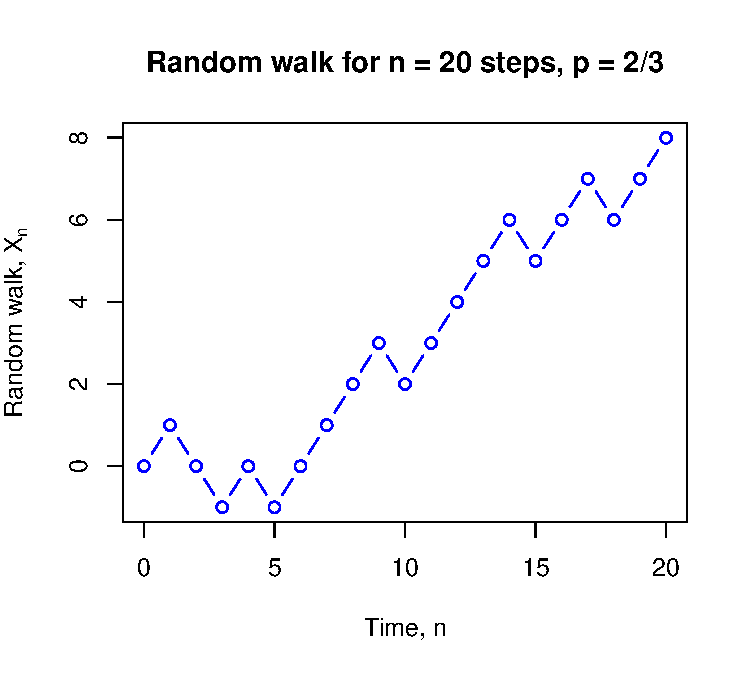
\includegraphics[width=0.5\linewidth]{math2750_files/figure-latex/rw-pics-1} 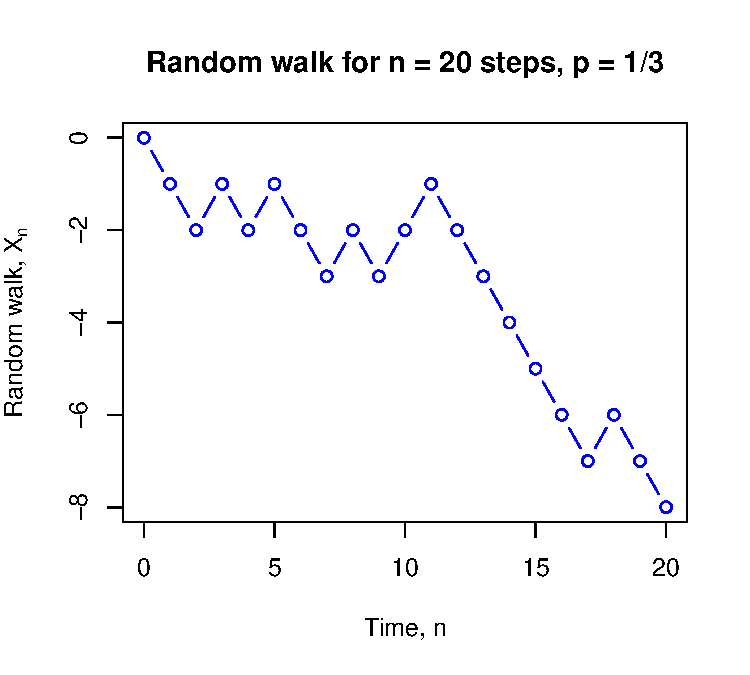
\includegraphics[width=0.5\linewidth]{math2750_files/figure-latex/rw-pics-2} \caption{Two simulations of random walks.}\label{fig:rw-pics}
\end{figure}

We can write this as a stochastic process \((X_n)\) with discrete time \(n = \{0,1,2,\dots\} = \mathbb Z_+\) and discrete state space \(\mathcal S = \mathbb Z\), where \(X_0 = 0\) and, for \(n \geq 0\), we have
\[ X_{n+1} = \begin{cases} X_n + 1 & \text{with probability $p$,} \\
                             X_n - 1 & \text{with probability $q$.} \end{cases} \]

It's clear from this definition that \(X_{n+1}\) (the future) depends on \(X_n\) (the present), but, given \(X_n\), does not depend on \(X_{n-1}, \dots, X_1, X_0\) (the past). Thus the Markov property holds, and the simple random walk is a \textbf{discrete time Markov process} or \textbf{Markov chain}.

\begin{example}
\protect\hypertarget{exm:rw1}{}\label{exm:rw1}

\emph{What is the probability that after two steps a simple random walk has reached \(X_2 = 2\)?}

To achieve this, the walk must go upwards in both time steps, so \(\mathbb P(X_2 = 2) = pp = p^2\).

\end{example}

\begin{example}
\protect\hypertarget{exm:rw2}{}\label{exm:rw2}

\emph{What is the probability that after three steps a simple random walk has reached \(X_3 = -1\)?}

There are three ways to reach \(-1\) after three steps: up--down--down, down--up--down, or down--down--up. So
\[ \mathbb P(X_3 = -1) = pqq+qpq+qqp = 3pq^2 . \]

\end{example}

\hypertarget{general-random-walks}{%
\subsection{General random walks}\label{general-random-walks}}

An alternative way to write the simple random walk is to put
\begin{equation}
    X_n = X_0 + \sum_{i=1}^n Z_i ,  \label{eq:rw}
  \end{equation}
where the starting point is \(X_0 = 0\) and the \textbf{increments} \(Z_1, Z_2, \dots\) are independent and identically distributed (IID) random variables with distribution given by \(\mathbb P(Z_i = 1) = p\) and \(\mathbb P(Z_i = -1) = q\). You can check that \eqref{eq:rw} means that \(X_{n+1} = X_n + Z_{n+1}\), and that this property defines the simple random walk.

Any stochastic process with the form \eqref{eq:rw} for some \(X_0\) and some distribution for the IID \(Z_i\)s is called a \textbf{random walk} (without the word ``simple'').

Random walks often have state space \(\mathcal S = \mathbb Z\), like the simple random walk, but they could be defined on other state spaces. We could look at higher dimensional simple random walks: in \(\mathbb Z^2\), for example, we could step up, down, left or right each with probability \(\frac14\). We could even have a continuous state space like \(\mathbb R\), if, for example, the \(Z_i\)s had a normal distribution.

We can use this structure to calculate the expectation or variance of any random walk (including the simple random walk).

Let's start with the expectation. For a random walk \((X_n)\) we have
\[ \mathbb E X_n = \mathbb E \left(X_0 + \sum_{i=1}^n Z_i\right) = \mathbb E X_0 + \sum_{i=1}^n \mathbb E Z_i = \mathbb EX_0 + n \mathbb E Z_1 , \]
where we've used the linearity of expectation, and that the \(Z_i\)s are identically distributed.

In the case of the simple random walk, we have \(\mathbb E X_0 = 0\), since we start from \(0\) with certainty, and
\[ \mathbb E Z_1 = \sum_{z \in \mathbb Z} z \mathbb P(Z_1 = z) = 1\times p + (-1)\times q = p-q .\]
Hence, for the simple random walk, \(\mathbb EX_n = n(p-q)\).

If \(p > \frac12\), then \(p > q\), so \(\mathbb E X_n\) grows ever bigger over time, while if \(p < \frac12\), then \(\mathbb E X_n\) grows ever smaller (that is, negative with larger absolute value) over time. If \(p = \frac12 = q\), which is the case of the simple symmetric random walk, then then the expectation \(\mathbb E X_n = 0\) is zero for all time.

Now the variance of a random walk. We have
\[ \operatorname{Var}(X_n) = \operatorname{Var}\left(X_0 + \sum_{i=1}^n Z_i\right) = \operatorname{Var}X_0 + \sum_{i=1}^n \operatorname{Var}Z_i = \operatorname{Var}X_0 + n \operatorname{Var}Z_1 , \]
where it was crucial that \(X_0\) and all the \(Z_i\)s were independent (so we had no covariance terms).

For the simple random walk we have \(\operatorname{Var}X_0 = 0\), since we always start from \(0\) with certainty. To calculate the variance of the increments, we write
\begin{align*}
  \operatorname{Var}(Z_1) &= \mathbb E (Z_1 - \mathbb EZ_1)^2 \\
            &= p\big(1 - (p-q)\big)^2 + q \big( {-1} - (p-q)\big)^2\\
            &= p(2q)^2 + q(-2p)^2\\
            &= 4pq^2 + 4p^2q \\
            &= 4pq(p+q) \\
            &= 4pq .
  \end{align*}
Here we've used that \(1-p = q\), \(1-q=p\), and \(p+q = 1\); you should take a few moments to check you've followed the algebra here. Hence the variance of the simple random walk is \(4pqn\). We see that (unless \(p\) is \(0\) or \(1\)) the variance grows over time, so it becomes harder and harder to predict where the random walk will be.

The variance of the simple symmetric random walk is \(4 \frac12 \frac12 n = n\).

For large \(n\), we can use a normal approximation for a random walk. Suppose the increments process \((Z_n)\) has mean \(\mu\) and variance \(\sigma^2\), and that the walk starts from \(X_0 = 0\). Then we have \(\mathbb E X_n = \mu n\) and \(\operatorname{Var}(X_n) = \sigma^2 n\), so for large \(n\) we can use the normal approximation \(X_n \approx \mathrm{N}(\mu n, \sigma^2 n)\). (Remember, of course, that the \(X_n\) are not independent.) To be more formal, the central limit theorem tells us that, as \(n \to \infty\), we have
\[ \frac{X_n - n\mu}{\sigma \sqrt{n}} \to \mathrm{N}(0,1) . \]

\hypertarget{exact-distribution}{%
\subsection{Exact distribution of the simple random walk}\label{exact-distribution}}

In the case of the simple random walk, we can in fact give the exact distribution by writing down an exact formula for \(\mathbb P(X_n = i)\) for any time \(n\) and any state \(i\).

Recall that, at each of the first \(n\) times, we independently take an upward step with probability \(p\), and otherwise take a downward step. So if we let \(Y_n\) be the number of upward steps over the first \(n\) time periods, we see that \(Y_n\) has a binomial distribution \(Y_n \sim \text{Bin}(n,p)\).

Recall that the binomial distribution has probability
\[  \mathbb P(Y_n = k)  = \binom nk p^k (1-p)^{n-k} = \binom nk p^k q^{n-k} , \]
for \(k = 0,1,\dots, n\), where \(\binom{n}{k}\) is the binomial coefficient ``\(n\) choose \(k\)''.

If \(Y_n = k\), that means we've taken \(k\) upward steps and \(n-k\) downward steps, leaving us at position \(k - (n-k) = 2k - n\). Thus we have that
\begin{equation}
  \mathbb P(X_n = 2k - n) = \mathbb P(Y_n = k) = \binom nk p^k q^{n-k} .  \label{eq:bin}
  \end{equation}

Note that after an odd number of time steps \(n\) we're always at an odd-numbered state, since \(2k - \text{odd} = \text{odd}\), while after an even number of time steps \(n\) we're always at an even-numbered state, since \(2k - \text{even} = \text{even}\).

Writing \(i = 2k - n\) gives \(k = (n+i)/2\) and \(n-k = (n-i)/2\). So we can rearrange \eqref{eq:bin} to see that the distribution for the simple random walk is
\[ \mathbb P(X_n = i) =  \binom{n}{(n+i)/2} p^{(n+i)/2} q^{(n-i)/2} , \]
when \(n\) and \(i\) have the same parity with \(-n \leq i \leq n\), and is \(0\) otherwise.

In the special case of the simple symmetric random walk, we have
\[ \mathbb P(X_n = i) = \binom{n}{(n+i)/2} \left(\frac12\right)^{(n+i)/2} \left(\frac12\right)^{(n-i)/2} = \binom{n}{(n+i)/2} 2^{-n} . \]

\textbf{In the next section}, we look at a gambling problem based on the simple random walk.

\hypertarget{P01}{%
\section*{Problem Sheet 1}\label{P01}}
\addcontentsline{toc}{section}{Problem Sheet 1}

You should attempt all these questions and write up your solutions in advance of your workshop in week 2 (Monday 1 or Tuesday 2 February) where the answers will be discussed.

\textbf{1.} When designing a model for a quantity that changes over time, one has many decisions to make:

\begin{itemize}
\tightlist
\item
  Discrete or continuous state space?
\item
  Discrete or continuous index set for time?
\item
  Deterministic or stochastic model?
\item
  If a stochastic model is chosen, is it reasonable to assume that the Markov property holds?
\end{itemize}

What would you decide for the following scenarios:

\textbf{(a)} The percentage of US voters with a positive opinion of Donald Trump in the Gallup weekly tracking poll.

\textbf{(b)} The number of points won by a football league club throughout the season.

\textbf{(c)} The temperature of a bowl of water placed in an oven.

\textbf{(d)} The number of people inside the Chemistry building.

\begin{myanswers}

\emph{Suggestions.} This question is meant to inspire discussion, so there are not necessarily right and wrong answers. If I were designing the models, however, my choices might be these:

\textbf{(a)} Discrete space if percentages are given to nearest 1\%, otherwise continuous; discrete time (weekly); stochastic; the Markov property might be appropriate, perhaps using some sort of random walk.

\textbf{(b)} Discrete space (number of points); discrete time (update after each game); stochastic; the Markov property might be appropriate, depending on if you think teams can have non-Markovian ``winning streaks'' (or losing streaks) that don't reflect underlying performance.

\textbf{(c)} Continuous space (temperature); continuous time; if the oven is reliable and the experiment carried out carefully, a deterministic model might be sufficient.

\textbf{(d)} Discrete space (number of people); continuous time; stochastic; Markov property might not be appropriate due to `bursts' of people leaving during fire drills or lectures finishing early.

\end{myanswers}

\textbf{2.} A fair six-sided dice is rolled twice, resulting in the
values \(X_1, X_2 \in \{1, 2, \ldots, 6\}\). Let \(Y = X_1 + X_2\) be the total score.
Calculate:

\textbf{(a)} the probability \(\mathbb P(Y = 10)\);

\begin{myanswers}

\emph{Solution.} The following table illustrates the possible outcomes \(Y\) of the experiment. Each cell of the table is an equally probable outcome.

\begin{center}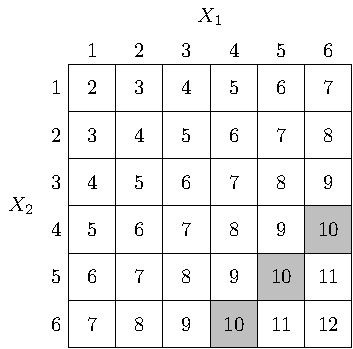
\includegraphics{math2750_files/figure-latex/dice-1} \end{center}

There are 3 possible ways to get \(Y=10\) (the grey cells in the table) out of the \(36\) possible outcomes, so we have \(\mathbb P(Y = 10) = 3/36 = 1/12\).

\end{myanswers}

\textbf{(b)} the conditional probability \(\mathbb P(Y=10 \mid X_1=x)\) for \(x=1, 2, \ldots, 6\);

\begin{myanswers}

\emph{Solution.} Conditioning on \(X_1 = x\) means restricting our attention only to column \(x\) of the table. Each column has \(6\) equally probably cells. For \(x=1,2,3\), none of the entries equal \(10\), so \(\mathbb P(Y=10 \mid X_1=x) = 0/6 = 0\). For each of \(x=4,5,6\), one of the entries equals \(10\), so \(\mathbb P(Y=10 \mid X_1=x) = 1/6\).

\end{myanswers}

\textbf{(c)} the conditional probability \(\mathbb P(X_1=x \mid Y=10)\) for \(x=1, 2, \ldots, 6\).

\begin{myanswers}

\emph{Solution.} Conditioning on \(Y =10\) means restricting our attention only to the \(3\) shaded cells, which are each equally likely. For \(x=1,2,3\), none of the shaded cells are in column \(x\), so \(\mathbb P(X_1=x \mid Y=10) = 0/3 = 0\). For each of \(x=4,5,6\), one of the shaded cells is in column \(x\), so \(\mathbb P(X_1=x \mid Y=10) = 1/3\).

\end{myanswers}

\textbf{3.} Let \((X_n)\) be a simple random walk starting from \(X_0 = 0\) and that at each step goes up one with probability \(p\) or down one with probability \(q = 1-p\). What are:

\textbf{(a)} \(\mathbb P(X_5 = 3)\),

\begin{myanswers}

\emph{Solution.} To get \(X_5 = 3\), we must take \(4\) steps up and \(1\) step down. The down step can be at any of the \(5\) time steps. Therefore we have \(\mathbb P(X_5 = 3) = 5p^4q\).

\end{myanswers}

\textbf{(b)} \(\mathbb P(X_5 = 3 \mid X_2 = 2)\),

\begin{myanswers}

\emph{Solution.} Once we're at \(X_2 = 2\), we must take \(2\) steps up and \(1\) step down over the next \(3\) time steps. So \(\mathbb P(X_5 = 3 \mid X_2 = 2) = 3p^2q\).

\end{myanswers}

\textbf{(c)} \(\mathbb P(X_n = n-2)\),

\begin{myanswers}

\emph{Solution.} This requires \(n-1\) steps up and \(1\) step down, and the down step can be at any of the \(n\) time steps. So \(\mathbb P(X_n = n-2) = np^{n-1}q\).

\end{myanswers}

\textbf{(d)} \(\mathbb E X_4\),

\begin{myanswers}

\emph{Solution.} The increments \(Z_n = X_n - X_{n-1}\) have expectation \(1p + (-1)q = p - q\), so \(\mathbb E X_4 = 4(p-q)\).

\end{myanswers}

\textbf{(e)} \(\mathbb E(X_6 \mid X_4 = 2)\),

\begin{myanswers}

\emph{Solution.} We are already at 2, then another two increments will take us up \(2(p-q)\) on average. Therefore \(\mathbb E(X_6 \mid X_4 = 2) = 2 + 2(p-q)\).

\end{myanswers}

\textbf{4.} The price \(X_n\) of a stock at the close of day \(n\) is modelled as a Gaussian random walk, where the increments \((Z_n)\) have a normal distribution \(Z_n \sim \text{N}(\mu, \sigma^2)\). The model assumes a drift of \(\mu = 0.7\) and a volatility of \(\sigma = 2.2\). The initial price is \(X_0 = 42.3\).

\textbf{(a)} Calculate the mean and variance of the price of the stock at the close of day \(5\).

\begin{myanswers}

\emph{Solution.} The mean and variance are
\begin{gather*}
  \mathbb EX_5 = \mathbb E X_0 + n \mathbb E Z_1 = 42.3 + 5 \cdot 0.7 = 45.8 , \\
  \operatorname{Var}X_5 = \operatorname{Var}X_0 + n \operatorname{Var}Z_1 = 0 + 5 (2.2)^2 = 24.2 .
  \end{gather*}

\end{myanswers}

\textbf{(b)} Give a 95\% prediction interval for the price at the close of day 5. (You might find it useful to recall that, if \(W \sim \text{N}(0,1)\) is a standard normal random variable, then \(\mathbb P(W \leq 1.96) = 0.975\).)

\begin{myanswers}

\emph{Solution.} Note that \(X_5\) itself is normally distributed, so \(X_5 \sim \text{N}(45.8,24.2)\). The 95\% prediction interval for a normal distribution \(\text{N}(\mu, \sigma^2)\) is \((\mu - 1.96\sigma, \mu + 1.96\sigma)\), so the prediction interval for \(X_5\) is
\[ \big(45.8 - 1.96\sqrt{24.2},  45.8 + 1.96\sqrt{24.2}\big) = (36.16, 55.44) . \]

\end{myanswers}

\textbf{(c)} After day 4, the prices at the end of each of the first four days have been recorded as \(X_1 = 44.4, X_2 = 44.0, X_3 = 47.1, X_4 = 47.8\). Update your prediction interval for the price at the close of day 5, and comment on how it differs from the earlier prediction interval.

\begin{myanswers}

\emph{Solution.} By the Markov property, \(X_5\) depends on \(X_4\), but given \(X_4\) does not depend on the other values, which we can therefore ignore. Since \(X_5 = X_4 + Z_5\), we have
\begin{gather*}
  \mathbb E(X_5 \mid X_4) = X_4 + \mathbb E Z_5 = 47.8 + 0.7 = 48.5 \\
  \operatorname{Var}(X_5 \mid X_4) = 0 + \operatorname{Var}Z_5 = 0 + (2.2)^2 = 4.84.
  \end{gather*}
The desired prediction interval is
\[ \big(48.5 - 1.96\sqrt{4.84},  48.5+ 1.96\sqrt{4.84}\big) = (44.19, 52.81) . \]
Compared to before, the centre of the prediction interval is slightly higher, because the stock has outperformed expectations so far, and the interval is much narrower, because as we get closer to day 5 we become less uncertain.

\end{myanswers}

\textbf{5.} A gambler decides to model her total winnings as a simple random walk starting from \(X_0 = 0\) that at each time goes up one with probability \(p\) and down one with probability \(1-p\), but where \(p\) is unknown. The first \(10\) recordings, \(X_1\) to \(X_{10}\), are
\[ (1, 2, 1, 2, 3, 4, 5, 6, 5, 6) . \]

\textbf{(a)} What would you guess for the value of \(p\), given this data?

\begin{myanswers}

\emph{Solution.} In \(10\) time steps, the process went up \(k = 8\) times and down \(n - k = 2\) times. So it seems reasonable to guess that \(p\) has the value \(\hat p = 8/10 = 0.8\).

\end{myanswers}

\textbf{(b)} More generally, how would you estimate \(p\) from the data \(X_0 = 0, X_1 = x_1, X_2 = x_2, \dots, X_n = x_n\)?

\begin{myanswers}

\emph{Solution.} We will estimate \(\hat p = k/n\), where \(k\) is the number of upward steps. We saw in lectures that \(k = (n + x_n)/2\), so our estimate is
\[ \hat p = \frac{n + x_n}{2n} = \frac12\ + \frac{x_n}{2n} . \]

\end{myanswers}

\textbf{(c)} Show that your estimate is in fact the maximum likelihood estimate of \(p\).

\begin{myanswers}

\emph{Solution.} You could answer this question by using what you know about maximum likelihood estimation for the binomial distribution from MATH1712, but we'll reason from first principles here.

If we let \(k\) be the number of upward steps, then the likelihood is
\[ f(\mathbf x; p) = p^{k}(1-p)^{n-k} , \]
making the the log-likelihood
\[ \ell(\mathbf x; p) = \ln f(\mathbf x; p) = k \ln p + (n-k)\ln(1-p) .\]
We maximise this by differentiating and setting equal to \(0\). The derivative is
\[ \frac{\text{d}}{\text{d}p} \ell(\mathbf x; p) = \frac kp - \frac{n-k}{1-p} ,\]
so the maximum likelihood estimate \(\hat p\) satisfies
\[ 0 = \frac k{\hat p} - \frac{n-k}{1-\hat p} . \]
Solving this by clearing denominators we get
\[ 0 = (k - k\hat p) - (n\hat p - k\hat p) = k - n \hat p , \]
and rearranging gives \(\hat p = k/n\) as desired.

\end{myanswers}

\end{document}
